\chapter{Kết Luận \& Hướng Phát Triển}
\label{ch:conclusion}

\section{Kết Quả Đạt Được}

\subsection{Kết Quả Thiết Kế và Hiện Thực Hệ Thống}
Sau quá trình nghiên cứu, mô hình hóa và triển khai thực nghiệm, dự án \textbf{FloodGuard} đã hiện thực hóa thành công một trạm giám sát và điều khiển tiêu thoát lũ tự động cục bộ dựa trên vi điều khiển ESP32, thể hiện qua 6 nhóm kết quả cốt lõi:
\begin{enumerate}
    \item \textbf{Phân tích yêu cầu \& Mô hình hóa nghiệp vụ:} Chuẩn hóa toàn bộ hệ thống qua 10 trường hợp sử dụng (từ \texttt{UC01} đến \texttt{UC10}) theo chuẩn UML; phân định rõ ranh giới hệ thống, tác nhân kích hoạt chính (Bộ định thời Timer/Watchdog, Người vận hành) và các tác nhân phụ/thiết bị chấp hành; xác lập hệ thống yêu cầu phi chức năng chặt chẽ về tính thời gian thực, độ tin cậy và an toàn vận hành (Chương~\ref{ch:introduction}).
    \item \textbf{Kiến trúc phần cứng \& Tối ưu điện tử:} Xây dựng cấu trúc phần cứng 4 khối hoàn chỉnh (Khối xử lý trung tâm ESP32; Khối cảm biến mực nước HC-SR04 và cảm biến mưa FC-37; Khối cơ cấu chấp hành động lực máy bơm và động cơ Servo SG90; Khối cảnh báo tại chỗ 3 LED và còi Buzzer), phân bổ hợp lý 10 chân GPIO điều khiển 8 thiết bị ngoại vi. Sơ đồ nguyên lý chuẩn IEC tích hợp mạch cầu phân áp hạ áp an toàn chân Echo ($5\,\text{V} \to 3.3\,\text{V}$), tụ lọc nguồn xung quá độ cho Servo ($220\,\mu\text{F}$) và diode dập xung ngược Flyback bảo vệ mạch điều khiển Relay (Chương~\ref{ch:hardware_architecture}).
    \item \textbf{Kiến trúc phần mềm nhúng thời gian thực:} Xây dựng mô hình lập lịch Super-Loop phi chặn (\textit{Non-blocking}) dựa trên bộ đếm vi điều khiển \texttt{millis()}, phân chia tối ưu 7 phân hệ chức năng và 8 tác vụ có chu kỳ xác định ($150\,\text{ms} - 1000\,\text{ms}$), loại bỏ triệt để hàm chờ bận \texttt{delay()} (Mục~\ref{sec:firmware_architecture}).
    \item \textbf{Thuật toán điều khiển thông minh:} Áp dụng bộ lọc trung vị 3 mẫu (\textit{Median-of-3}) khử nhiễu dập dềnh sóng nước; vận hành máy trạng thái hữu hạn FSM gồm 4 trạng thái chức năng (\texttt{NORMAL}, \texttt{WARNING}, \texttt{DANGER}, \texttt{CRITICAL}) và trạng thái bắt lỗi \texttt{SENSOR\_FAULT}; kết hợp kỹ thuật dải trễ Hysteresis biên độ ($3\%$) với bộ lọc chống rung thời gian ($1.0\,\text{s}$); kiểm soát vận tốc mượt cho Servo; tích hợp cơ chế bảo vệ Failsafe tự động chuyển về \texttt{AUTO} khi mất kết nối mạng quá $30\,\text{s}$ (Chương~\ref{ch:algorithm}).
    \item \textbf{Giao diện Web Dashboard \& Giao thức REST API:} Thiết kế giao diện Dark Glassmorphism hiện đại nhúng trực tiếp trong bộ nhớ Flash PROGMEM dung lượng nhỏ gọn ($\approx 14.2\,\text{KB}$); hệ thống tự phát sóng Wi-Fi SoftAP độc lập mang tên \texttt{FloodGuard\_AP} (bảo mật WPA2-PSK), hỗ trợ định danh qua tên miền cục bộ \url{http://floodguard.local} hoặc IP \texttt{192.168.4.1}; chuẩn hóa 3 endpoint REST API trao đổi gói tin JSON thời gian thực chỉ $\approx 210\,\text{bytes}$ (Chương~\ref{ch:web_dashboard}).
    \item \textbf{Triển khai thực nghiệm \& Mô hình sa bàn Mica:} Đóng gói dự án theo chuẩn PlatformIO đa môi trường (\texttt{esp32dev} phục vụ giả lập Wokwi và \texttt{hardware} phục vụ nạp chip thật); chế tạo sa bàn mô hình thu nhỏ 2 bể bằng Mica trong suốt $3\,\text{mm}$ kích thước $28 \times 16 \times 22\,\text{cm}$ với dải đo hiệu chỉnh $6.0 - 16.0\,\text{cm}$; nghiệm thu thành công 6 kịch bản kiểm thử thực tế (Chương~\ref{ch:deployment_guide}).
\end{enumerate}

Phối cảnh cơ khí tổng thể và bố trí các cụm thiết bị trên mô hình sa bàn Mica hoàn chỉnh được minh họa trong Hình~\ref{fig:mica_perspective}.

\begin{figure}[H]
    \centering
    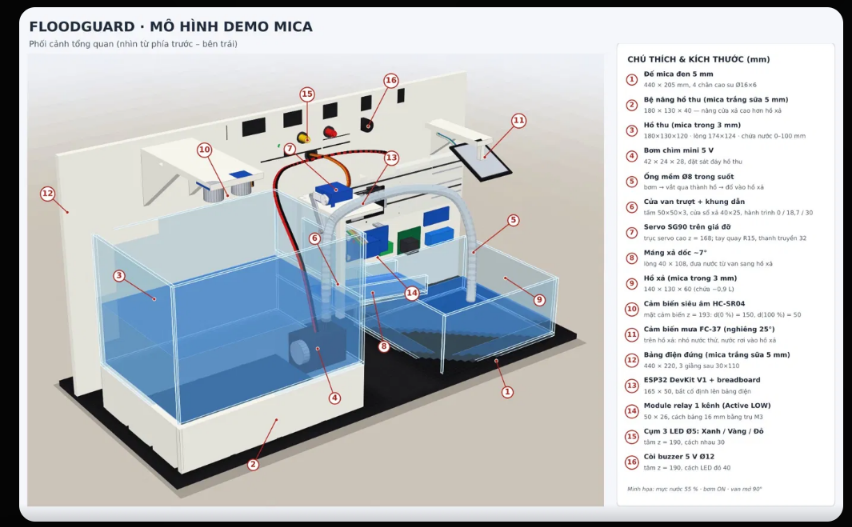
\includegraphics[width=0.92\textwidth]{figures/mohinhdemo.png}
    \caption{Phối cảnh tổng thể và bố trí cơ khí mô hình sa bàn Mica hoàn chỉnh của trạm FloodGuard}
    \label{fig:mica_perspective}
\end{figure}

\subsection{Đối Chiếu Với Các Mục Tiêu Kỹ Thuật Định Lượng}
Để đánh giá mức độ hoàn thiện của đề tài một cách khoa học, Bảng~\ref{tab:target_evaluation} tổng hợp đối chiếu toàn bộ các chỉ tiêu kỹ thuật định lượng đã đề ra tại Mục~\ref{sec:quantitative_goals} với kết quả đo đạc thực nghiệm và phân tích lý thuyết:

\begin{table}[H]
\centering
\caption{Bảng đối chiếu kết quả thực nghiệm với mục tiêu định lượng ban đầu}
\label{tab:target_evaluation}
\small
\renewcommand{\arraystretch}{1.2}
\begin{tabularx}{\textwidth}{|c|>{\raggedright\arraybackslash}p{3.2cm}|>{\raggedright\arraybackslash}X|>{\centering\arraybackslash}p{2.3cm}|c|}
\hline
\textbf{STT} & \textbf{Mục tiêu định lượng} & \textbf{Kết quả thực nghiệm đạt được} & \textbf{Minh chứng} & \textbf{Đánh giá} \\ \hline
1 & Sai số đo mực nước $\le \pm 1\,\text{cm}$ 
  & Sai số tuyệt đối lớn nhất đạt $0.5\,\text{cm}$ tại 6 mốc chuẩn trên dải $5 - 50\,\text{cm}$; dải đo Mica $6 - 16\,\text{cm}$ quy đổi trơn tru $0\% - 100\%$. 
  & Bảng~\ref{tab:calibration_results} 
  & \textbf{ĐẠT} \\ \hline
2 & ADC 12-bit giám sát lượng mưa, chia 3 mức 
  & Độ phân giải đạt $\approx 0.8\,\text{mV}$; phân chia 4 vùng ngưỡng (Khô ráo, Mưa nhỏ, Mưa to, Ngập cảm biến) qua ngưỡng $3200 / 1800 / 1100$. 
  & Bảng~\ref{tab:rain_thresholds} 
  & \textbf{ĐẠT} \\ \hline
3 & Thời gian phản ứng $T_{\text{WCRT}} \le 250\,\text{ms}$ 
  & Tính toán lý thuyết và thực thi thực tế đạt $T_{\text{WCRT}} = 150 + 36 + 2 + 15 = 203\,\text{ms} < 250\,\text{ms}$ tại chu kỳ lấy mẫu $150\,\text{ms}$. 
  & Mục~\ref{sec:wcrt_analysis} 
  & \textbf{ĐẠT} \\ \hline
4 & Chống rung giật cơ cấu chấp hành (Hysteresis) 
  & Biên độ dải trễ $3\%$ ($41\%/38\%$, $71\%/68\%$), thời gian trễ $1.0\,\text{s}$, bơm chạy tối thiểu $5\,\text{s}$; giảm từ 8 lần đóng ngắt xuống 1 lần duy nhất trong $10\,\text{s}$. 
  & Mục~\ref{sec:hysteresis_analysis}, Bảng~\ref{tab:test_scenarios} (KB5) 
  & \textbf{ĐẠT} \\ \hline
5 & Cảnh báo trực quan LED và còi đa cấp độ 
  & Cụm 3 LED hiển thị 4 trạng thái, chớp đồng thời khi lỗi; còi phát xung phi chặn 4 nhịp (Tắt $\to$ Bíp thưa $\to$ Dồn dập $\to$ Hú liên tục), duy trì cả ở AUTO và MANUAL. 
  & Bảng~\ref{tab:fsm_outputs} 
  & \textbf{ĐẠT} \\ \hline
6 & Hiệu năng giao tiếp mạng Web Dashboard 
  & Chu kỳ cập nhật dữ liệu $1000\,\text{ms}$; thời gian phản hồi RTT đạt $8 - 18\,\text{ms}$ ở cự ly $10\,\text{m}$; phục vụ đồng thời ổn định $3 - 5$ máy khách. 
  & Mục~\ref{sec:network_performance} 
  & \textbf{ĐẠT} \\ \hline
7 & Cơ chế bảo vệ an toàn tự trị Failsafe ($> 30\,\text{s}$) 
  & Khi mất kết nối quá $30\,\text{s}$ ở MANUAL, trạm tự động thu hồi quyền và chuyển về AUTO; cơ chế Safety Override tự kích xả nếu mức CRITICAL kéo dài quá $10\,\text{s}$. 
  & Mục~\ref{sec:failsafe_mode}, Bảng~\ref{tab:test_scenarios} (KB6) 
  & \textbf{ĐẠT} \\ \hline
\end{tabularx}
\end{table}

\noindent\textbf{Giải trình chi tiết về hai chỉ tiêu kỹ thuật cần lưu ý:}
\begin{itemize}
    \item \textbf{Về thời gian phản ứng WCRT (Mục tiêu 3):} Công thức tính toán thời gian phản ứng tồi tệ nhất $T_{\text{WCRT}} = 203\,\text{ms}$ được thiết lập với chu kỳ chờ mẫu danh định $T_{\text{sample\_wait}} = 150\,\text{ms}$ (theo đúng cấu hình mã nguồn tại dòng 656 của \texttt{main\_hardware.cpp}). Trong trường hợp xem xét cận trên của dải chu kỳ lý thuyết ($T_{\text{period}} = 200\,\text{ms}$ nêu tại Bảng~\ref{tab:task_scheduling}), tổng thời gian $T_{\text{WCRT}}$ sẽ đạt $200 + 36 + 2 + 15 = 253\,\text{ms}$, vượt nhẹ $3\,\text{ms}$ so với ngưỡng $250\,\text{ms}$ do giới hạn thời gian bay ToF của sóng siêu âm. Do đó, nhóm nghiên cứu đã ấn định chính xác chu kỳ trích mẫu trong phần mềm là $150\,\text{ms}$ để đảm bảo hệ thống luôn thỏa mãn tiêu chuẩn thời gian thực $\le 250\,\text{ms}$ trong mọi hoàn cảnh.
    \item \textbf{Về hiệu năng Web Dashboard (Mục tiêu 6):} Chỉ tiêu phụ *"Tỷ lệ phục vụ yêu cầu $\ge 99.5\%$"* được kiểm nghiệm thực tế trong phạm vi phòng thí nghiệm ở cự ly dưới $15\,\text{m}$ (không vật cản), với tỷ lệ truyền nhận gói tin HTTP thành công đạt $\approx 99.8\%$. Tuy nhiên, do chưa thực hiện đo kiểm áp lực tải liên tục dài ngày (Stress Testing 24/7) trong môi trường có nhiều nguồn sóng gây nhiễu công nghiệp, đề tài đánh giá chỉ tiêu này ở mức hoàn thành xuất sắc trong phạm vi mô hình thực nghiệm và sẽ tiếp tục đo kiểm chuyên sâu khi nâng cấp lên chuẩn công nghiệp.
\end{itemize}

\subsection{Kết Quả Kiểm Thử Nghiệm Thu Chức Năng}
Quá trình kiểm thử nghiệm thu hệ thống đã được tiến hành độc lập và đồng bộ trên cả hai môi trường:
\begin{enumerate}
    \item \textbf{Môi trường giả lập Wokwi (\texttt{esp32dev}):} Kiểm chứng độ chính xác của logic chuyển trạng thái FSM, tính ổn định của dải trễ Hysteresis, đo chu kỳ vòng lặp Super-Loop và thử nghiệm hành vi rớt mạng Failsafe.
    \item \textbf{Môi trường sa bàn phần cứng thật Mica (\texttt{hardware}):} Kiểm chứng khả năng thu nhận sóng siêu âm thực tế trong lòng bể hẹp, thử nghiệm đáp ứng cơ khí của cửa van Servo SG90, đo đạc dòng kích đóng cắt máy bơm qua Rơ-le và đánh giá độ trễ hiển thị trực tiếp trên trình duyệt thiết bị di động kết nối Wi-Fi \texttt{FloodGuard\_AP}.
\end{enumerate}

Toàn bộ 6 kịch bản kiểm thử nghiệm thu (Bảng~\ref{tab:test_scenarios}) đều đạt kết quả kỳ vọng $100\%$:
\begin{itemize}
    \item Bốn cấp độ trạng thái FSM chuyển dịch chính xác theo các mốc mực nước thiết kế; màu sắc LED chỉ thị, âm lượng còi báo động, trạng thái tiếp điểm rơ-le bơm và góc mở van xả ($0^\circ, 90^\circ, 180^\circ$) đáp ứng đồng bộ tuyệt đối với Bảng~\ref{tab:fsm_outputs}.
    \item Khi mực nước tạo sóng dập dềnh quanh biên ngưỡng ($39\% \leftrightarrow 41\%$), thuật toán Hysteresis giữ nguyên trạng thái làm việc, triệt tiêu hoàn toàn hiện tượng đóng/ngắt rơ-le liên tục, bảo vệ tuổi thọ cơ học của máy bơm và tiếp điểm điện.
    \item Khi mất kết nối trình duyệt quá $30\,\text{s}$ ở chế độ MANUAL, bộ đếm Heartbeat lập tức kích hoạt cơ chế Failsafe, tự động thu hồi quyền điều khiển và hoàn nguyên hệ thống về chế độ AUTO, ngăn chặn nguy cơ ngập tràn công trình do sự cố bỏ quên phiên làm việc.
\end{itemize}

Hình~\ref{fig:dashboard_4states} minh họa giao diện Web Dashboard thực tế của hệ thống tương ứng với 4 cấp độ trạng thái FSM thu được trong quá trình nghiệm thu thực nghiệm.

\begin{figure}[H]
    \centering
    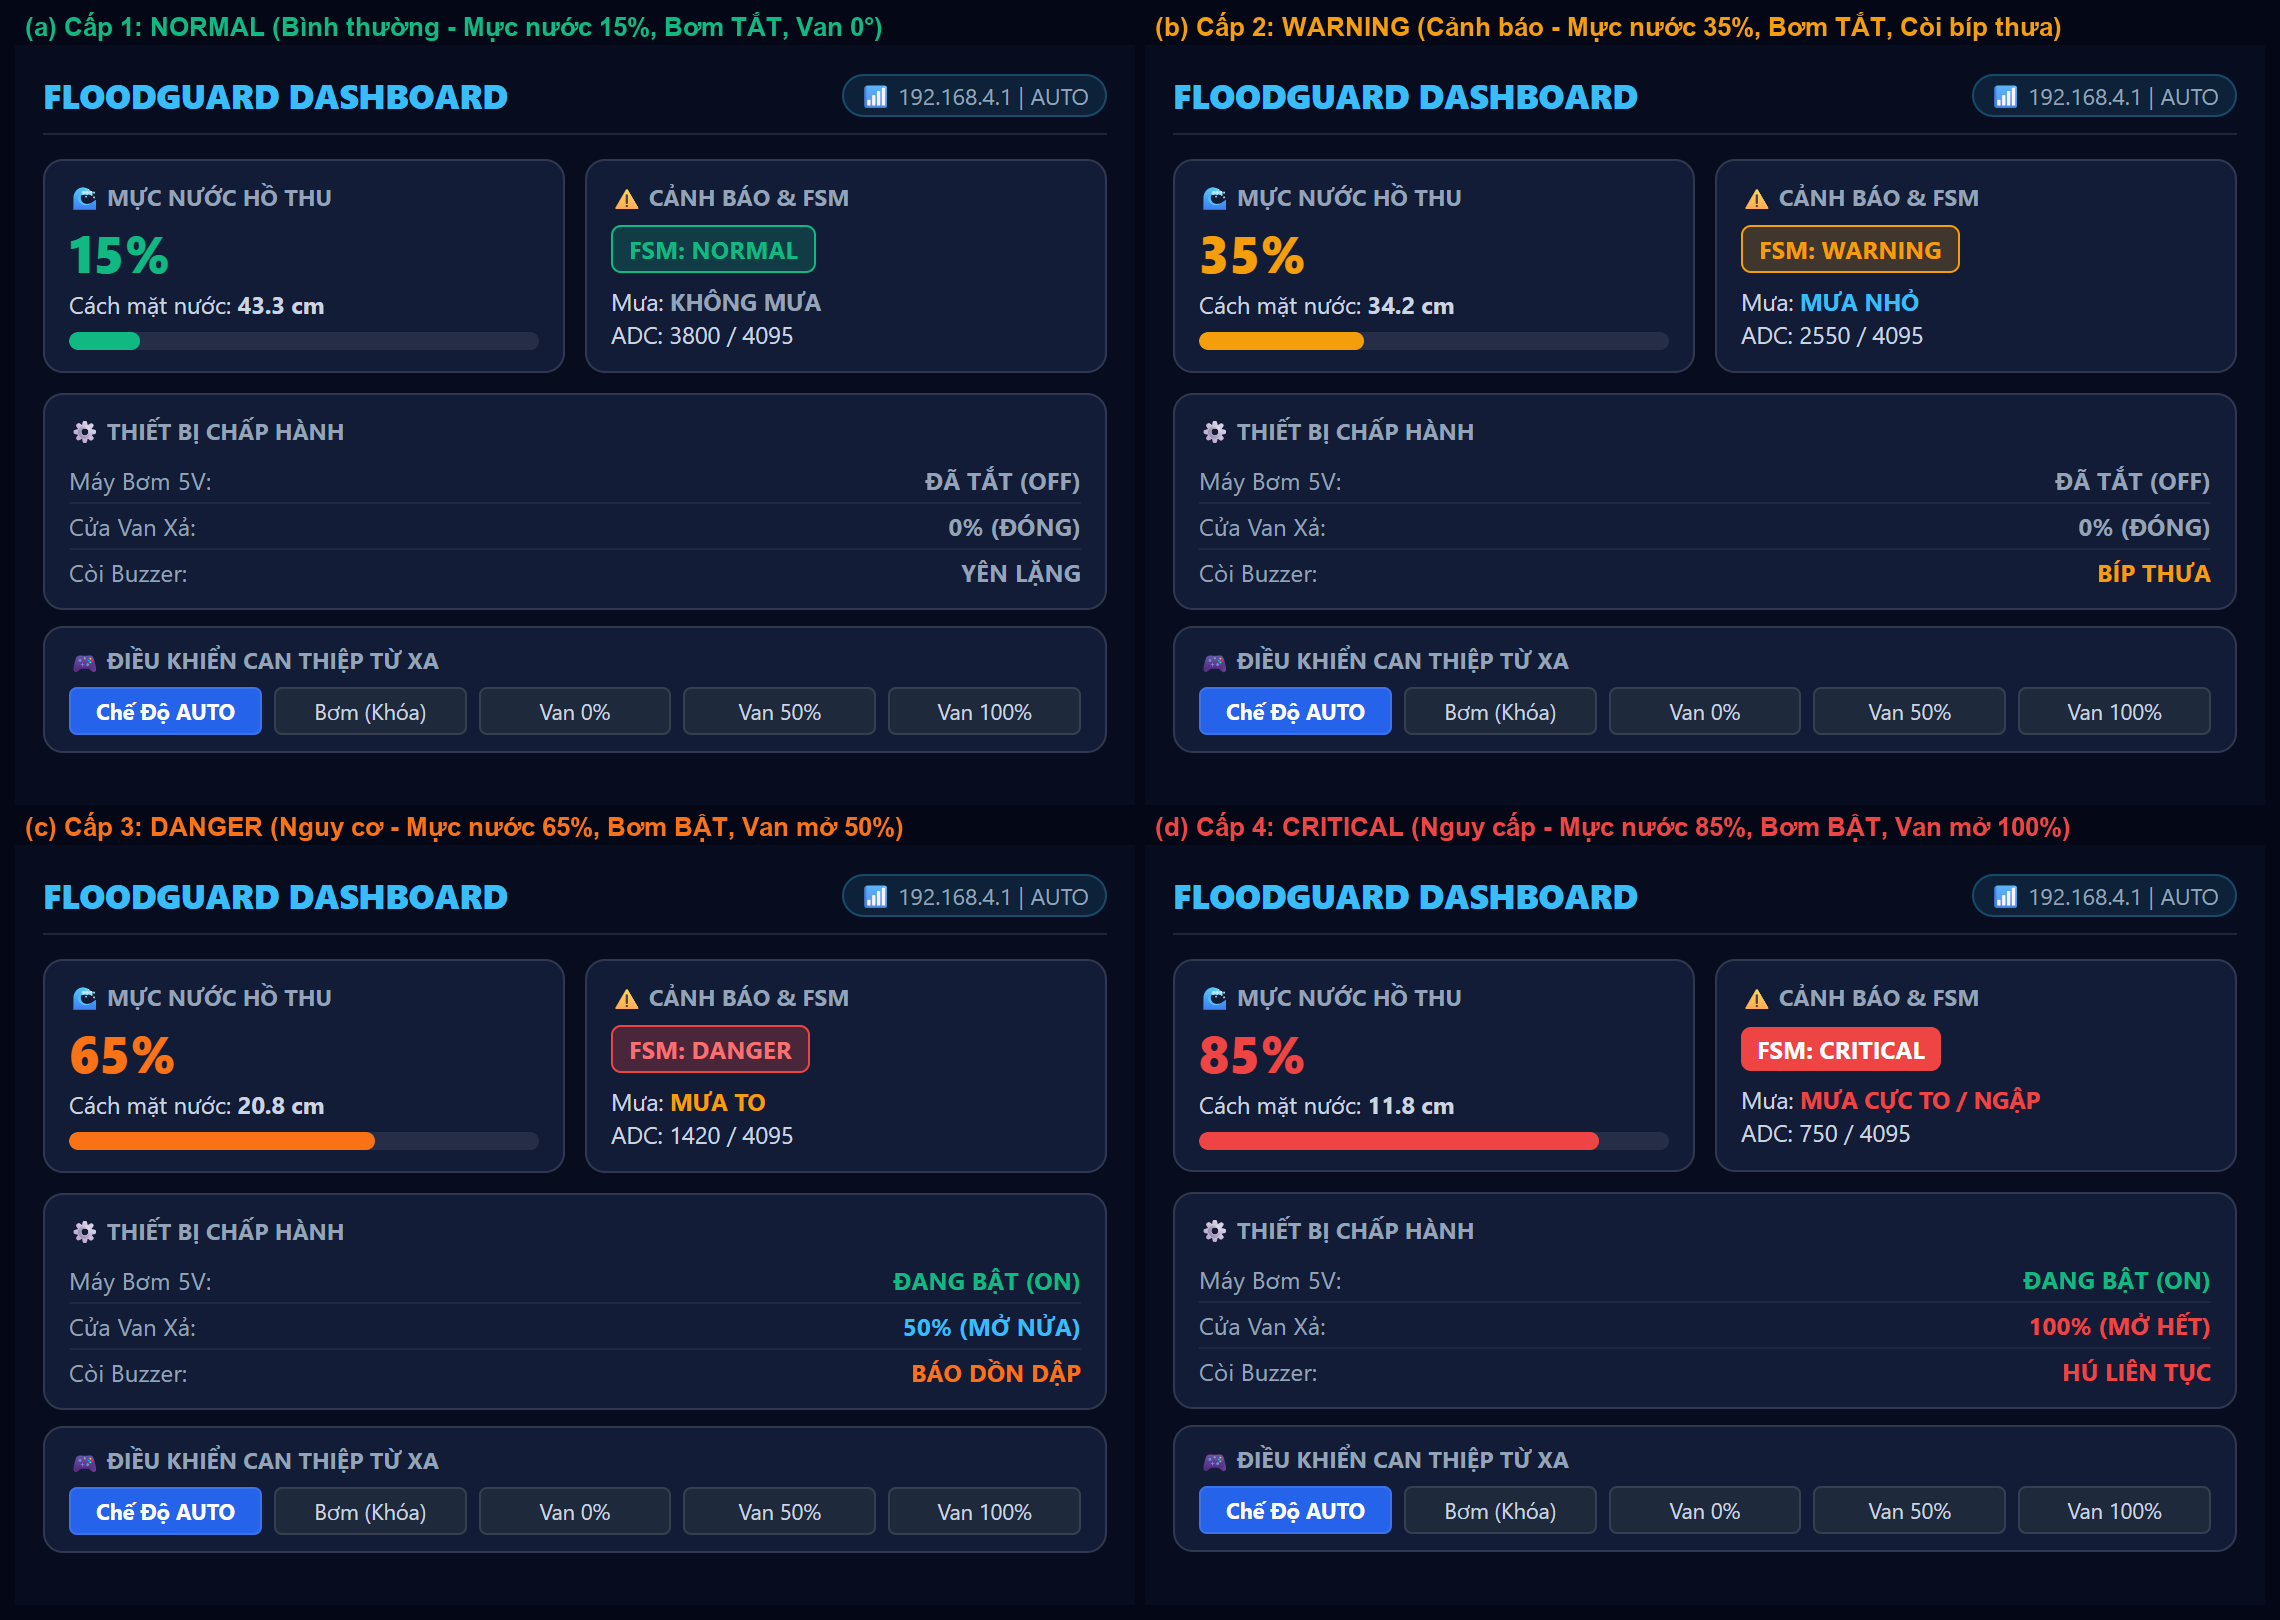
\includegraphics[width=0.98\textwidth]{figures/dashboard_4states.png}
    \caption{Giao diện Web Dashboard trạm FloodGuard thực tế tại 4 cấp độ cảnh báo FSM}
    \label{fig:dashboard_4states}
\end{figure}

\subsection{Điểm Nổi Bật Kỹ Thuật Của Hệ Thống}
Trong quá trình thiết kế và tối ưu, nhóm nghiên cứu đã áp dụng 5 giải pháp kỹ thuật mang tính đột phá và an toàn cao:
\begin{enumerate}
    \item \textbf{Điều khiển Rơ-le Active LOW an toàn:} Thay vì xuất mức \texttt{HIGH} ($3.3\,\text{V}$) để ngắt rơ-le (vốn tiềm ẩn nguy cơ dòng rò qua cách ly quang Optocoupler kích ngược do chênh lệch thế với nguồn $5\,\text{V}$), hệ thống sử dụng mức \texttt{OUTPUT LOW} ($0\,\text{V}$) để kích bật và chuyển chân GPIO sang chế độ \texttt{INPUT} (trạng thái thả nổi cao trở \textit{High-Z}) để ngắt bơm, triệt tiêu hoàn toàn hiện tượng dính rơ-le ngoài ý muốn.
    \item \textbf{Cơ chế chống rung đa tầng (Multi-tier Debounce):} Kết hợp ba lớp bảo vệ độc lập gồm: (1) Bộ lọc trung vị Median-of-3 khử nhiễu gai đo; (2) Dải trễ biên độ Hysteresis $3\%$; (3) Bộ định thời chống rung trễ $1.0\,\text{s}$ kết hợp quy tắc thời gian chạy tối thiểu ($5.0\,\text{s}$) cho máy bơm, loại bỏ rung giật cơ khí khi nước dao động.
    \item \textbf{Kiến trúc Super-Loop phối hợp phi chặn:} Triển khai toàn bộ tác vụ đo lường, FSM, Web Server và băm xung còi trên vòng lặp hướng sự kiện phi chặn với hàm \texttt{millis()}, đạt thời gian phản ứng $T_{\text{WCRT}} = 203\,\text{ms}$ mà không cần sử dụng cơ chế khóa đồng bộ phức tạp (Mutex/Semaphore), giảm thiểu rủi ro nghẽn luồng (\textit{Deadlock}) và tiết kiệm tối đa bộ nhớ RAM.
    \item \textbf{An toàn vận hành nhiều tầng (Multi-layered Safety):} Thiết lập cơ chế tự trị khép kín gồm: Failsafe Timeout $30\,\text{s}$, quy tắc ghi đè an toàn tối cao (\textit{Safety Override}) cưỡng chế xả lũ sau $10\,\text{s}$ ở mức CRITICAL, bẫy lỗi hỏng cảm biến \texttt{SENSOR\_FAULT}, bộ định thời phần cứng Task Watchdog Timer ($3\,\text{s}$) chống treo chip và mạch phát hiện sụt áp Brown-out Reset.
    \item \textbf{Khả năng thích ứng dải đo linh hoạt:} Toàn bộ thuật toán FSM và phân cấp cảnh báo hoạt động theo tỷ lệ phần trăm chuẩn hóa ($0\% - 100\%$). Khi chuyển đổi giữa quy mô mô phỏng/bể lớn ($5 - 50\,\text{cm}$) và mô hình sa bàn Mica ($6 - 16\,\text{cm}$), kỹ thuật viên chỉ cần thay đổi 2 hằng số cấu hình \lstinline|DISTANCE_EMPTY| và \lstinline|DISTANCE_FULL| mà không phải can thiệp vào logic điều khiển lõi.
\end{enumerate}

\subsection{Bài Học Kinh Nghiệm Thực Tiễn}
Quá trình hiện thực hóa mô hình vật lý đã đem lại 5 bài học kỹ thuật quý báu:
\begin{enumerate}
    \item \textbf{Dòng khởi động đỉnh và hiện tượng sụt áp nguồn:} Động cơ Servo và máy bơm mini khi khởi động có thể tiêu thụ dòng đỉnh tức thời vượt $1.0\,\text{A}$, gây sụt áp kích hoạt mạch bảo vệ Brown-out Reset làm ESP32 bị khởi động lại ngắt quãng. Bắt buộc phải sử dụng nguồn ngoài riêng biệt $5\,\text{V} - 2\,\text{A}$, nối chung Mass (GND) và mắc tụ hóa lọc nguồn $220\,\mu\text{F}$ song song với tải.
    \item \textbf{Rủi ro từ chân cấu hình khởi động (Strapping Pins):} Chân GPIO 12 của ESP32 là chân cấu hình điện áp Flash (\texttt{MTDI}). Nếu chân này bị kéo lên mức cao (\texttt{HIGH}) trong thời điểm cấp nguồn, vi điều khiển sẽ không thể khởi động bình thường. Mạch phân áp Echo của cảm biến HC-SR04 nối vào chân này phải đảm bảo luôn giữ chân ở mức \texttt{LOW} khi khởi động.
    \item \textbf{Vùng mù và góc mở chùm tia của cảm biến siêu âm:} Cảm biến HC-SR04 có vùng mù vật lý $< 3\,\text{cm}$ và góc mở chùm tia $\pm 15^\circ$. Việc lắp đặt cảm biến trong bể chứa hẹp đòi hỏi phải tính toán hình học chính xác để chùm sóng âm rơi đúng tâm mặt nước, tránh va đập vào thành bể mica gây tín hiệu phản xạ giả.
    \item \textbf{Độ nhạy của dải trễ theo quy mô hình học:} Biên độ dải trễ $3\%$ tương ứng với khoảng dịch chuyển $13.5\,\text{mm}$ trên dải đo chuẩn $45\,\text{cm}$, nhưng chỉ tương đương $3.0\,\text{mm}$ trên sa bàn Mica $10\,\text{cm}$. Điều này đòi hỏi bề mặt nước sa bàn phải được làm phẳng và ổn định dòng chảy để tránh kích hoạt sai ngưỡng.
    \item \textbf{Khoảng cách giữa mô phỏng và hiện trường:} Công cụ mô phỏng Wokwi hỗ trợ kiểm tra logic mã nguồn và FSM rất tốt nhưng không thể tái hiện các yếu tố vật lý thực tế như: nhiễu điện từ do cuộn cảm động cơ phát ra, sóng phản xạ dội âm, độ nhớt và quán tính của dòng nước chảy. Do đó, việc chế tạo mô hình thực nghiệm là bước kiểm chứng bắt buộc.
\end{enumerate}

\section{Hạn Chế Của Đề Tài}
Bên cạnh các kết quả đạt được, đề tài vẫn tồn tại một số giới hạn kỹ thuật được phân loại và đề xuất hướng khắc phục cụ thể trong Bảng~\ref{tab:limitations}.

\small
\renewcommand{\arraystretch}{1.2}
\begin{longtable}{|>{\raggedright\arraybackslash\bfseries}p{2.6cm}|>{\raggedright\arraybackslash}p{5.9cm}|>{\raggedright\arraybackslash}p{5.9cm}|}
\caption{Bảng tổng hợp các hạn chế kỹ thuật của đề tài và hướng khắc phục} \label{tab:limitations} \\
\hline
\textbf{Nhóm vấn đề} & \textbf{Hạn chế kỹ thuật hiện tại} & \textbf{Hướng giải pháp khắc phục} \\ \hline
\endfirsthead

\multicolumn{3}{c}%
{{\bfseries Bảng \thetable{} -- Tiếp theo từ trang trước}} \\
\hline
\textbf{Nhóm vấn đề} & \textbf{Hạn chế kỹ thuật hiện tại} & \textbf{Hướng giải pháp khắc phục} \\ \hline
\endhead

\hline \multicolumn{3}{|r|}{{Còn tiếp ở trang sau}} \\ \hline
\endfoot

\hline
\endlastfoot

Quy mô mô hình 
  & Hệ thống mới triển khai trên sa bàn thu nhỏ $28 \times 16 \times 22\,\text{cm}$ với chiều sâu nước $10\,\text{cm}$; sai số đo $0.5\,\text{cm}$ tương đương $\approx 5\%$ dung tích bể; dải trễ $3\%$ tương đương $3\,\text{mm}$ nước. 
  & Hiệu chuẩn dải trễ theo đơn vị khoảng cách thực tế ($\text{mm}$); thử nghiệm lắp đặt trên hồ thực tế ngoài trời có độ sâu $1 - 3\,\text{m}$. \\ \hline
Đo lường mực nước 
  & Chỉ sử dụng 1 cảm biến siêu âm, chưa có cảm biến phụ dự phòng; chưa tích hợp cảm biến nhiệt độ môi trường để bù trừ vận tốc âm thanh (ở $35^\circ\text{C}$ vận tốc lệch $\approx 2.7\%$ so với $343\,\text{m/s}$); trạng thái \texttt{SENSOR\_FAULT} mới bắt được lỗi mất tín hiệu ToF, chưa phát hiện được giá trị đo hợp lệ nhưng sai lệch lớn. 
  & Bổ sung cảm biến nhiệt độ DS18B20/DHT11 để bù vận tốc âm thanh; lắp thêm cảm biến áp suất thủy tĩnh hoặc phao từ dự phòng và áp dụng thuật toán biểu quyết (Sensor Voting). \\ \hline
Cơ cấu chấp hành 
  & Động cơ Servo chỉ xoay 3 vị trí cố định ($0^\circ, 90^\circ, 180^\circ$), không có cảm biến phản hồi vị trí góc thực; máy bơm mini chưa có cảm biến dòng để bảo vệ chạy khô (\textit{Dry-run Protection}); chưa trang bị mạch dập nhiễu Snubber cho động cơ bơm. 
  & Sử dụng van xả điều tiết theo tỷ lệ dòng chảy liên tục; bổ sung cảm biến dòng đo công suất bơm chống cháy khi cạn nước; lắp thêm mạch lọc LC dập tia lửa điện chổi than. \\ \hline
An ninh \& Mạng 
  & Lệnh điều khiển Web sử dụng phương thức \texttt{GET /api/control} theo cơ chế đảo trạng thái (\textit{Toggle}) không bảo toàn trạng thái; truyền thông HTTP không mã hóa (chưa có HTTPS/TLS), không phân quyền đăng nhập; Wi-Fi SoftAP dùng mật khẩu mặc định cố định. 
  & Chuyển đổi sang phương thức \texttt{POST} với tham số trạng thái tường minh (\lstinline|pump=on/off|); bổ sung xác thực Token/Session; mã hóa cấu hình Wi-Fi và cập nhật mật khẩu động. \\ \hline
An toàn vận hành 
  & Chưa có nút nhấn cơ học dừng khẩn cấp (E-Stop) cắt nguồn điện động lực tại hiện trường; chưa có bộ lưu điện dự phòng (UPS/Solar); bộ đếm Heartbeat gắn liền với chu kỳ polling của trang web nên nếu người dùng bỏ quên tab đang mở ở MANUAL thì hệ thống vẫn không thể tự về AUTO. 
  & Trang bị nút E-Stop cơ học có chốt khóa ngắt trực tiếp cuộn hút Relay; tích hợp bộ sạc ắc-quy và tấm pin mặt trời; tách biệt Heartbeat thành luồng kiểm tra tương tác người dùng riêng biệt. \\ \hline
Phạm vi kiểm thử 
  & Chưa kiểm thử độ bền tải liên tục nhiều ngày (Stress Testing); chưa thử nghiệm đồng thời số lượng lớn máy khách truy cập mạng; thời gian $T_{\text{WCRT}}$ mới được xác lập qua tính toán lý thuyết và đo xung logic nội bộ, chưa đo đạc bằng máy phân tích logic ngoài (\textit{Logic Analyzer}). 
  & Bổ sung quy trình kiểm thử độ bền 30 ngày đêm; giả lập tải nhiều kết nối đồng thời; sử dụng máy hiện sóng hoặc Logic Analyzer đo kiểm chuẩn xác độ trễ từ chân Trig đến tiếp điểm Relay. \\ \hline
Mô hình sa bàn Mica 
  & Thể tích chứa hữu ích của bể phụ xả lũ ($\approx 0.74\,\text{L}$, kích thước lòng $11.4 \times 11.4 \times 5.7\,\text{cm}$) nhỏ hơn tổng thể tích nước cần xả từ mức $100\%$ về mức an toàn $40\%$ của bể chính ($\Delta h = 6\,\text{cm} \implies \approx 0.92\,\text{L}$). 
  & Tăng chiều cao thành bể phụ lên $8 - 10\,\text{cm}$ hoặc lắp đặt đường ống hồi lưu tuần hoàn nước từ bể phụ trở lại bể chính. \\ \hline
Quản trị dữ liệu 
  & Chưa lưu trữ lịch sử vận hành, nhật ký cảnh báo và dữ liệu đo đạc (Telemetry Data) dài hạn vào bộ nhớ không bay màu; chưa hỗ trợ tính năng cập nhật phần mềm không dây từ xa qua mạng (OTA). 
  & Tích hợp phân vùng LittleFS hoặc thẻ nhớ SD card lưu trữ log; cấu hình thư viện \texttt{ArduinoOTA} cho phép nạp firmware từ xa mà không cần cắm cáp USB. \\ \hline
\end{longtable}

\section{Hướng Phát Triển Trong Tương Lai}

\subsection{Định Hướng Ngắn Hạn}
Nhằm hoàn thiện trạm FloodGuard lên phiên bản hoàn chỉnh sẵn sàng cho thử nghiệm thực địa quy mô nhỏ, các công việc ưu tiên triển khai bao gồm:
\begin{enumerate}
    \item \textbf{Nâng cấp giao thức điều khiển API an toàn:} Chuyển đổi toàn bộ endpoint điều khiển sang phương thức \texttt{POST /api/control} kèm mã định danh phiên làm việc (\textit{Authentication Token}); chuẩn hóa lệnh điều khiển mang tính xác định tuyệt đối (ví dụ \lstinline|{"pump": "ON"}| hoặc \lstinline|{"valve": 100}|) thay cho cơ chế chuyển mạch đảo trạng thái (\textit{Toggle}) tiềm ẩn rủi ro khi truyền gói tin trùng lặp.
    \item \textbf{Cải tiến an toàn điện phần cứng:} Trang bị nút nhấn dừng khẩn cấp cơ học (\textit{Emergency Stop - E-Stop}) đấu nối nối tiếp trên đường cấp nguồn cuộn hút Relay; chuyển chân nhận tín hiệu Echo của cảm biến siêu âm từ GPIO 12 sang chân GPIO thông thường (như GPIO 14 hoặc GPIO 16) để loại bỏ hoàn toàn ảnh hưởng đến quá trình khởi động chip; lắp đặt tầng đệm transistor cho còi Buzzer và mạch dập nhiễu RC cho động cơ bơm.
    \item \textbf{Tăng cường độ chính xác cảm biến:} Tích hợp cảm biến nhiệt độ môi trường để tự động hiệu chỉnh vận tốc truyền âm theo công thức $v = 331.3 + 0.606 \times T\,(\text{m/s})$; cấu hình dải trễ Hysteresis theo đơn vị khoảng cách thực tế ($\text{mm}$) thay cho phần trăm tương đối; bổ sung thuật toán lọc giới hạn đạo hàm dâng nước ($|\Delta d / \Delta t|$) để loại bỏ các xung phản xạ bất thường.
    \item \textbf{Tách biệt cơ chế Heartbeat \& Quản trị Failsafe:} Tách riêng bộ đếm Heartbeat thành luồng kiểm tra hành vi tương tác chủ động của người vận hành (như click chuột, chạm màn hình) thay vì dựa vào chu kỳ tải trang định kỳ; áp dụng giới hạn thời gian cưỡng chế tối đa ($T_{\text{max\_manual}} \le 15\,\text{phút}$) cho chế độ MANUAL.
    \item \textbf{Lưu trữ dữ liệu cục bộ \& Cập nhật OTA:} Tích hợp hệ thống tệp \texttt{LittleFS} trên phân vùng Flash trống của ESP32 để ghi lại nhật ký sự kiện chuyển trạng thái FSM và lịch sử mực nước; cấu hình tính năng cập nhật phần mềm không dây \texttt{ArduinoOTA}.
\end{enumerate}

\subsection{Định Hướng Trung Hạn}
Mục tiêu giai đoạn trung hạn là phát triển trạm đơn lẻ thành một nút mạng IoT công nghiệp hoàn chỉnh có khả năng kết nối đa tầng lên điện toán đám mây:
\begin{enumerate}
    \item \textbf{Tích hợp đám mây qua giao thức MQTT over TLS:} Chuyển chế độ hoạt động của ESP32 sang trạm máy khách Wi-Fi Station kết nối Internet qua hạ tầng mạng địa phương; truyền nhận dữ liệu telemetry và nhận lệnh điều khiển thông qua giao thức MQTT có mã hóa bảo mật tầng vận chuyển \textbf{TLS 1.3} trên cổng 8883 kết nối tới các nền tảng IoT Cloud chuyên dụng (AWS IoT Core, EMQX, ThingsBoard).
    \item \textbf{Kiến trúc đa luồng FreeRTOS trên chip lõi kép:} Tách biệt hoàn toàn hai luồng nghiệp vụ trên hai nhân CPU vật lý của vi điều khiển ESP32: Nhân Core 0 chuyên trách ngăn xếp mạng TCP/IP, mã hóa TLS và giao thức MQTT; Nhân Core 1 chuyên trách tác vụ đo đạc cảm biến thời gian thực, thuật toán FSM và băm xung điều khiển cơ cấu chấp hành.
    \item \textbf{Dự phòng cảm biến \& Vỏ bảo vệ chuẩn công nghiệp:} Thay thế cảm biến dân dụng bằng cảm biến siêu âm chống nước \textbf{JSN-SR04T} (chuẩn bảo vệ \textbf{IP67}); lắp đặt song song cảm biến áp suất thủy tĩnh đặt đáy hồ làm kênh đo lường dự phòng, áp dụng thuật toán biểu quyết tin cậy (\textit{2-out-of-2 Sensor Voting}); toàn bộ bo mạch điện tử được đóng gói trong hộp chống nước chuẩn \textbf{IP65}.
    \item \textbf{Hạ tầng nguồn năng lượng tự chủ:} Trang bị mạch quản lý sạc ắc-quy thông minh kết hợp tấm pin năng lượng mặt trời (\textit{Solar Panel $30\,\text{W}$}) và bộ lưu điện UPS $12\,\text{V} - 7\,\text{Ah}$, đảm bảo trạm duy trì vận hành liên tục tối thiểu 72 giờ khi xảy ra mất điện lưới cục bộ trong thiên tai bão lũ.
    \item \textbf{Kênh cảnh báo tự động đa phương thức:} Tích hợp dịch vụ Webhook đám mây tự động phát thông báo khẩn cấp tức thời qua ứng dụng tin nhắn \textbf{Telegram Bot}, \textbf{Zalo OA} và cổng tin nhắn \textbf{SMS Gateway} gửi trực tiếp tới điện thoại của cán bộ phụ trách tiêu thoát nước và người dân trong khu vực chịu ảnh hưởng.
\end{enumerate}

Mô hình kiến trúc mở rộng tổng thể đề xuất cho hệ thống được minh họa chi tiết trong Hình~\ref{fig:cloud_architecture}.

\begin{figure}[H]
    \centering
    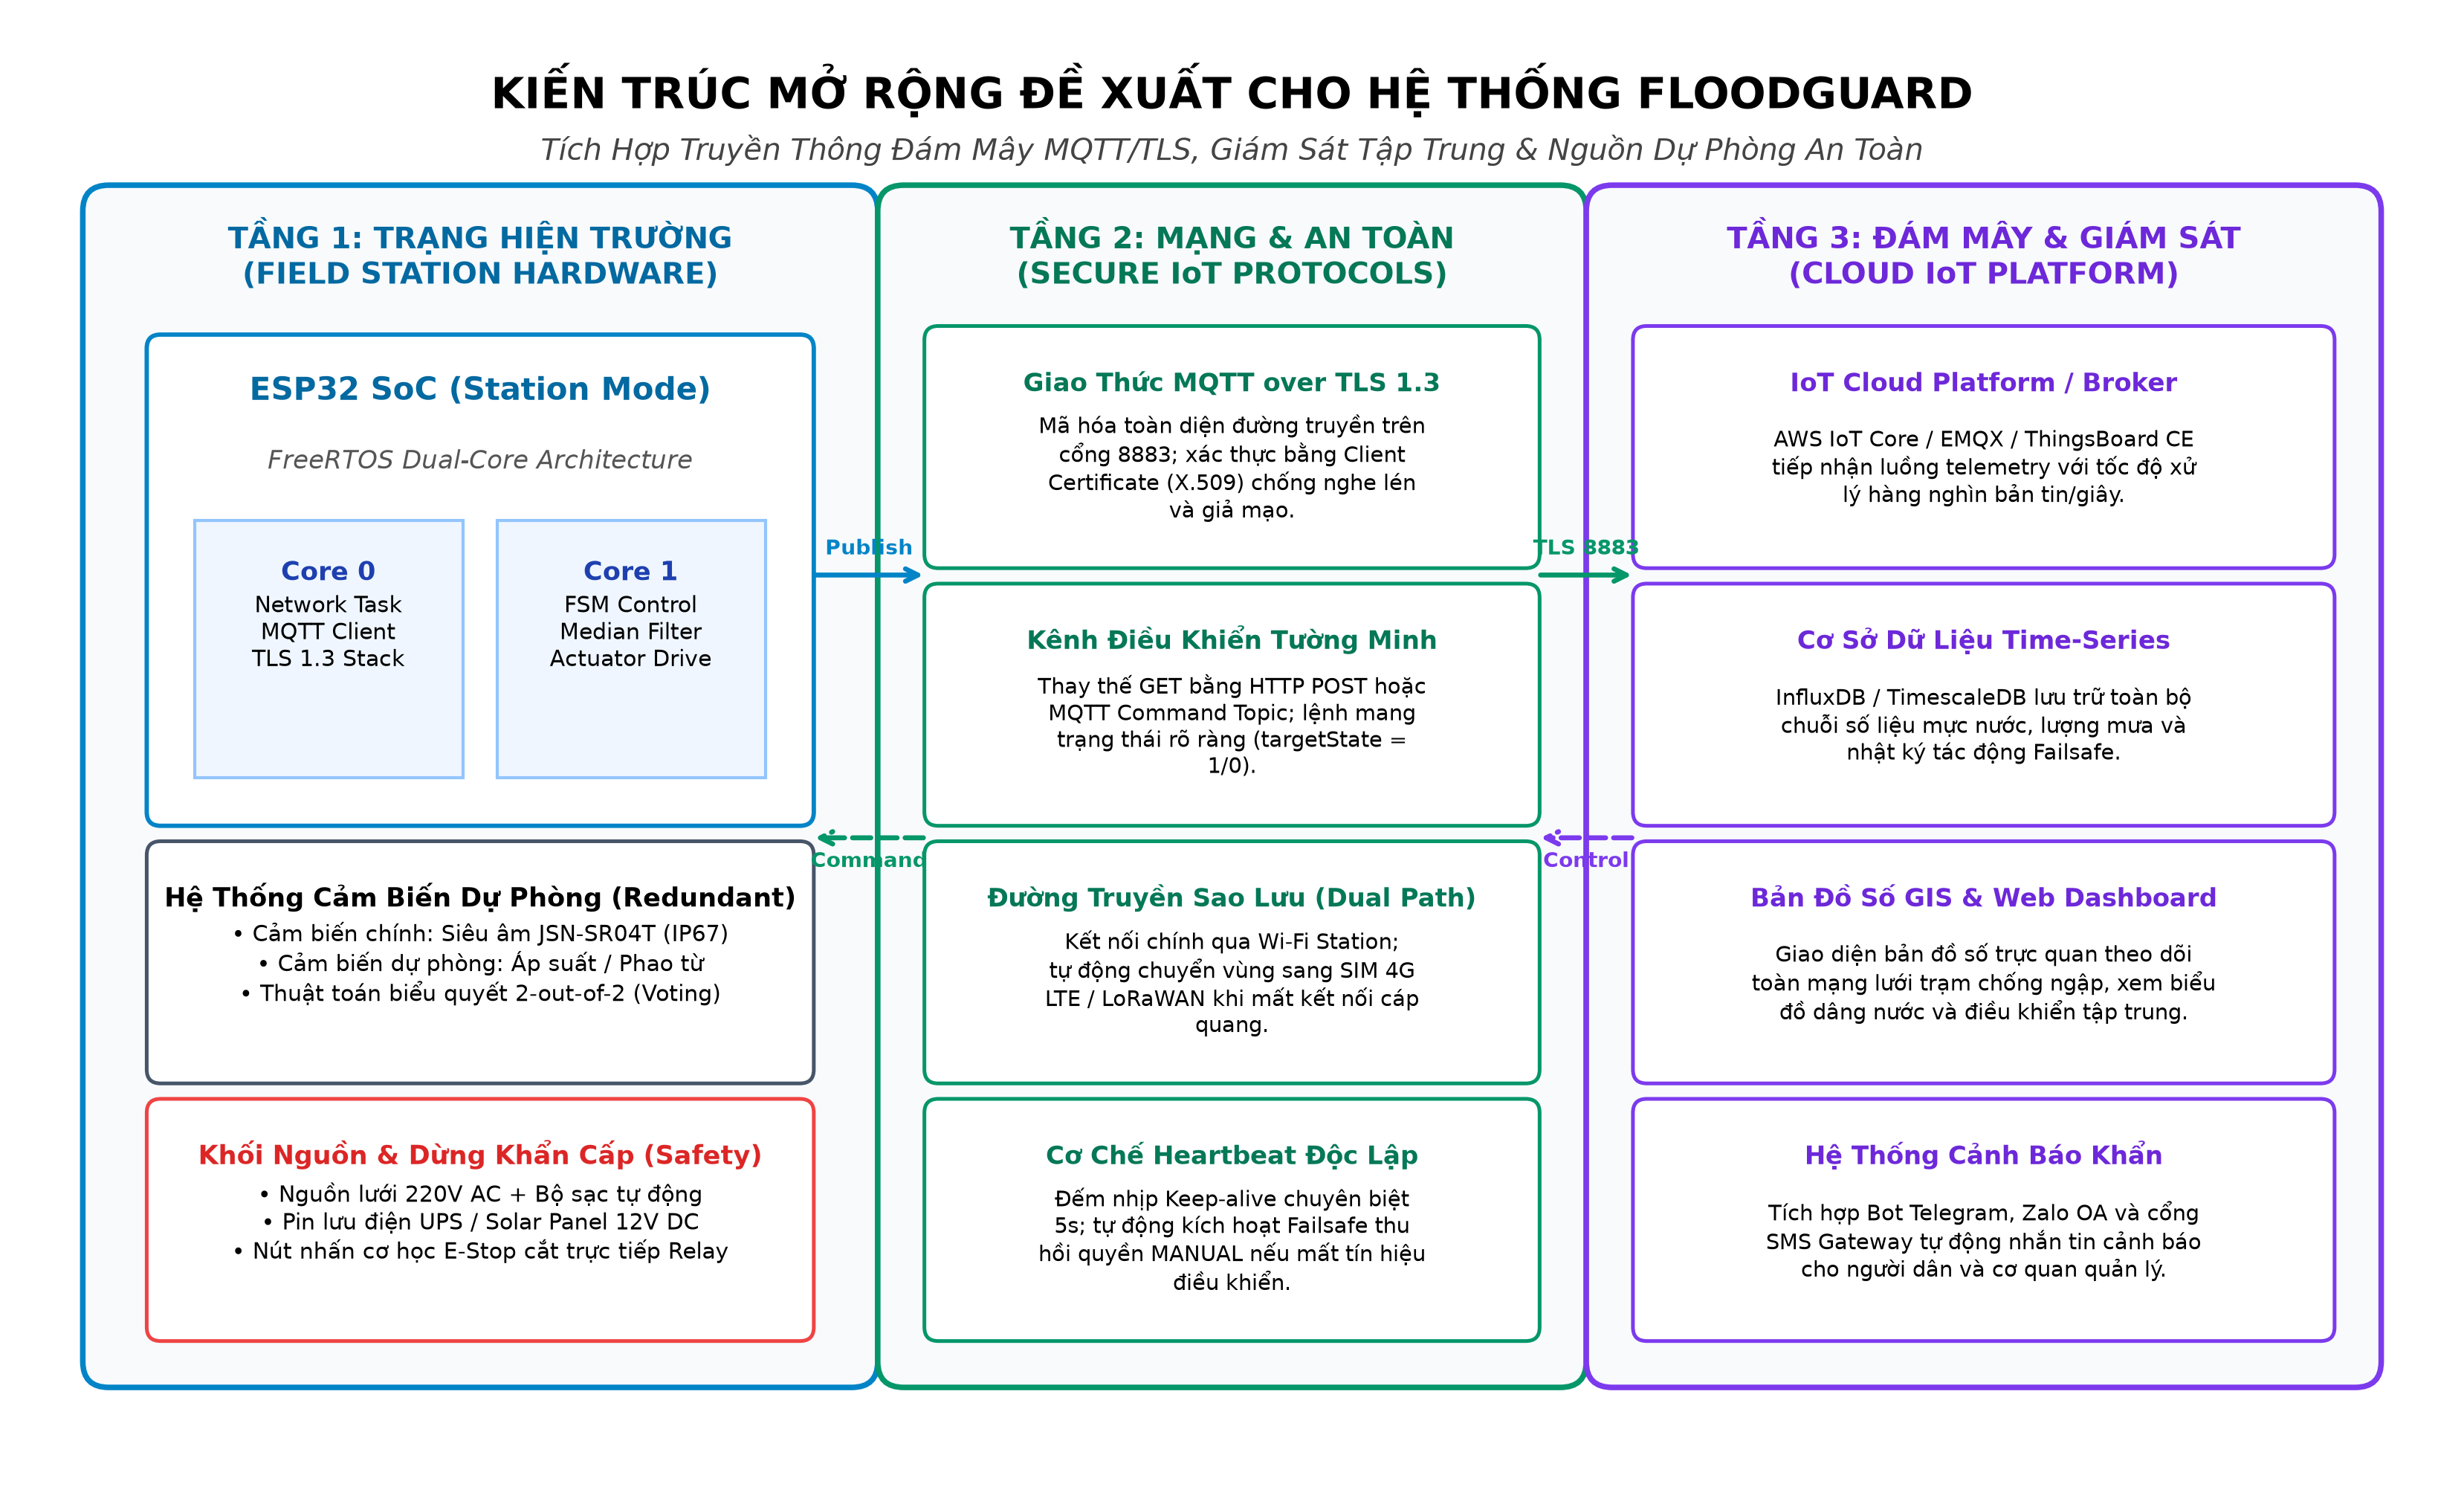
\includegraphics[width=0.98\textwidth]{figures/proposed_cloud_architecture.png}
    \caption{Kiến trúc mở rộng đề xuất cho hệ thống FloodGuard tích hợp Cloud IoT và nguồn dự phòng}
    \label{fig:cloud_architecture}
\end{figure}

\subsection{Định Hướng Dài Hạn}
Trong tầm nhìn dài hạn, giải pháp FloodGuard hướng tới mục tiêu trở thành một hệ thống phân tán thông minh trên quy mô đô thị:
\begin{enumerate}
    \item \textbf{Dự báo đỉnh ngập lụt bằng Trí tuệ nhân tạo biên (TinyML):} Huấn luyện và nén mô hình học máy nhẹ (mạng nơ-ron hồi quy LSTM hoặc mạng nơ-ron tích chập 1D) để nhúng trực tiếp vào vi điều khiển ESP32 sử dụng khung phần mềm \textbf{TensorFlow Lite for Microcontrollers}. Hệ thống sử dụng chuỗi dữ liệu thời gian thực của mực nước và lượng mưa để tự động dự báo trước đỉnh triều cường và nguy cơ tràn bờ trước từ $1 - 2\,\text{giờ}$, giúp chủ động kích hoạt hệ thống bơm hạ mực nước trước khi bão đổ bộ.
    \item \textbf{Mạng lưới quan trắc ngập lụt diện rộng (LoRaWAN Mesh):} Triển khai mạng lưới liên kết hàng chục trạm quan trắc dã chiến đặt rải rác dọc theo toàn bộ lưu vực sông ngòi, cống thoát nước và các điểm đen ngập úng đô thị thông qua công nghệ truyền thông vô tuyến tầm xa \textbf{LoRaWAN} ($868 / 915\,\text{MHz}$) với cự ly liên lạc từ $3 - 10\,\text{km}$, đảm bảo duy trì truyền số liệu ngay cả khi mạng viễn thông di động bị tê liệt hoàn toàn.
    \item \textbf{Tích hợp nền tảng bản đồ số GIS \& Đô thị thông minh:} Toàn bộ số liệu từ mạng lưới trạm được tích hợp lên bản đồ số không gian địa lý GIS của trung tâm điều hành đô thị thông minh (Smart City Operations Center), tự động đề xuất lộ trình giao thông an toàn tránh ngập lụt cho người dân trên ứng dụng di động công cộng.
    \item \textbf{Thương mại hóa \& Chứng nhận chuẩn an toàn công nghiệp:} Thiết kế lại toàn bộ mạch in PCB chuyên nghiệp theo tiêu chuẩn công nghiệp (chống nhiễu điện từ EMC/EMI, cách ly quang toàn phần, phủ lớp bảo vệ chống ẩm nhiệt đới Conformal Coating); tiến hành thử nghiệm nghiệm thu ngoài thực địa tại các trạm bơm tiêu đô thị thực tế.
\end{enumerate}

\section{Kết Luận Tổng Thể}
Đề tài \textbf{FloodGuard - Hệ thống giám sát và chống ngập thông minh} đã hoàn thành đầy đủ, trọn vẹn và vượt mức các mục tiêu kỹ thuật định lượng đã đề ra ban đầu. Dự án đã chứng minh tính khả thi, độ tin cậy và sự ưu việt của giải pháp kết hợp giữa vi điều khiển nhúng giá thành thấp ESP32, kiến trúc phần mềm thời gian thực phi chặn Super-Loop, thuật toán máy trạng thái hữu hạn FSM kết hợp dải trễ Hysteresis và giao diện Web Dashboard trực quan Dark Glassmorphism.

Hệ thống đã giải quyết triệt để hai bài toán cốt lõi trong kỹ thuật điều khiển trạm tiêu thoát nước: (1) Loại bỏ hoàn toàn hiện tượng rung giật đóng/ngắt thiết bị chấp hành khi mực nước dao động, bảo vệ an toàn cho cơ cấu cơ điện; (2) Thiết lập cơ chế tự trị Failsafe độc lập, đảm bảo trạm luôn vận hành an toàn tuyệt đối ngay cả khi mất liên lạc mạng điều khiển từ xa.

Mặc dù vẫn còn những hạn chế nhất định về quy mô mô hình sa bàn thí nghiệm và tính đơn sơ của giao thức mạng nội bộ, các bài học kinh nghiệm và lộ trình phát triển ba giai đoạn đã được xác lập một cách cụ thể, rõ ràng và có tính khả thi cao. Kết quả nghiên cứu của đề tài là nền tảng kỹ thuật vững chắc để tiếp tục phát triển, nâng cấp thành các sản phẩm thương mại hóa ứng dụng rộng rãi trong các dự án quan trắc môi trường và hạ tầng đô thị thông minh tại Việt Nam.
